\documentclass[aspectratio=169,11pt]{beamer}

\usetheme{Madrid}
\usecolortheme{default}
\setbeamertemplate{navigation symbols}{}
\setbeamertemplate{footline}[frame number]

\usepackage{amsmath,amssymb}
\usepackage{graphicx}
\usepackage{tikz}
\usetikzlibrary{positioning,calc}
\usetikzlibrary{arrows.meta,decorations.pathmorphing}

\definecolor{RamRed}{RGB}{190,40,45}
\definecolor{RamBlue}{RGB}{30,90,180}
\definecolor{SoftGray}{RGB}{245,245,245}
\definecolor{DarkGray}{RGB}{70,70,70}
\definecolor{MapGreen}{RGB}{48,150,95}
\definecolor{MapGold}{RGB}{235,180,45}

\setbeamercolor{title}{fg=DarkGray}
\setbeamercolor{frametitle}{fg=white,bg=RamBlue}
\setbeamercolor{structure}{fg=RamBlue}

\tikzset{
  v/.style={circle,draw=black,fill=white,inner sep=1.8pt},
  edge/.style={draw=RamBlue,line width=1.25pt},
  topic/.style={draw=black!30,fill=SoftGray,rounded corners=5pt,inner sep=7pt,
    text width=5.8cm,minimum height=1.65cm,align=left},
}


\usepackage{booktabs}
\tikzset{dot/.style={circle,fill=black,inner sep=2pt}, lab/.style={circle,draw=black,fill=white,inner sep=2pt,minimum size=6mm,font=\small},selected/.style={draw=RamRed,line width=2pt}}

\newcommand{\Def}[2]{\begin{block}{#1}#2\end{block}}
\newcommand{\Thm}[2]{\begin{block}{#1}#2\end{block}}
\renewcommand{\Proof}[1]{\begin{block}{Proof}\normalsize #1\end{block}}
\newcommand{\Question}[1]{\begin{block}{Question}#1\end{block}}
\renewcommand{\Example}[1]{\begin{block}{Example}#1\end{block}}
\newcommand{\fall}[2]{#1^{\underline{#2}}}
\newcommand{\rise}[2]{#1^{\overline{#2}}}
\newcommand{\stir}[2]{\left\{\begin{matrix}#1\\#2\end{matrix}\right\}}
\newcommand{\cyc}[2]{\left[\begin{matrix}#1\\#2\end{matrix}\right]}
\newcommand{\eul}[2]{\left\langle\begin{matrix}#1\\#2\end{matrix}\right\rangle}
\newcommand{\coef}[2]{[#1^{#2}]}
\newcommand{\gap}{\par\medskip}

\title{Colorings}
\author{Jeremy Quastel}\date{}\begin{document}
\begin{frame}[plain]\begin{center}{\Huge\bfseries Colorings}\par\vspace{.25cm}{\Large Section 1.6}\par\vspace{.15cm}{\large Harris--Hirst--Mossinghoff, \emph{Combinatorics and Graph Theory}}\par\vspace{.1cm}\resizebox{!}{2.7cm}{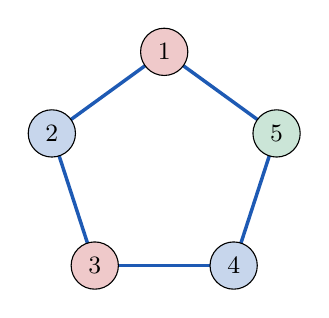
\begin{tikzpicture}[scale=1]
\coordinate (v1) at (0.000,1.500);
\coordinate (v2) at (-1.427,0.464);
\coordinate (v3) at (-0.882,-1.214);
\coordinate (v4) at (0.882,-1.214);
\coordinate (v5) at (1.427,0.464);
\draw[edge] (v1)--(v2);
\draw[edge] (v2)--(v3);
\draw[edge] (v3)--(v4);
\draw[edge] (v4)--(v5);
\draw[edge] (v5)--(v1);
\node[lab,fill=RamRed!25] at (v1) {1};
\node[lab,fill=RamBlue!25] at (v2) {2};
\node[lab,fill=RamRed!25] at (v3) {3};
\node[lab,fill=RamBlue!25] at (v4) {4};
\node[lab,fill=MapGreen!25] at (v5) {5};
\end{tikzpicture}}\par\vspace{.25cm}Jeremy Quastel\end{center}\end{frame}
\begin{frame}[plain]\large \begin{center}{\Huge\bfseries Today\textquotesingle s lecture}\par\vspace{.5cm}\end{center}\begin{columns}[c,onlytextwidth]\begin{column}{.48\textwidth}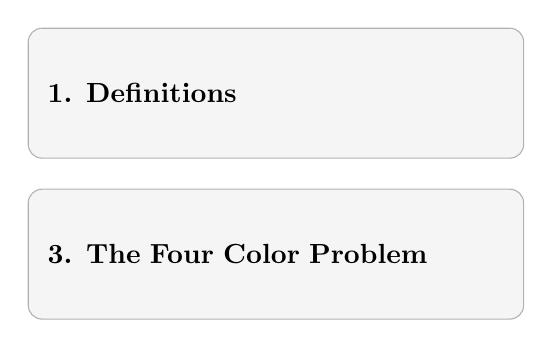
\begin{tikzpicture}\node[topic](a){\textbf{1. Definitions}};\node[topic,below=.38cm of a]{\textbf{3. The Four Color Problem}};\end{tikzpicture}\end{column}\begin{column}{.48\textwidth}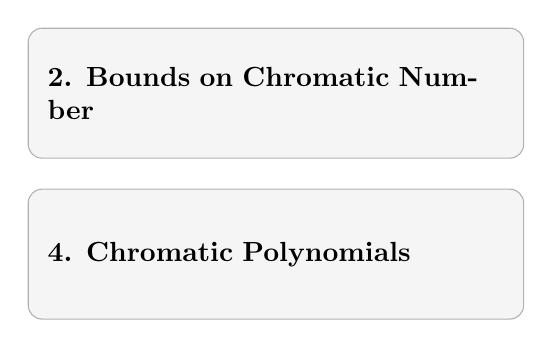
\begin{tikzpicture}\node[topic](a){\textbf{2. Bounds on Chromatic Number}};\node[topic,below=.38cm of a]{\textbf{4. Chromatic Polynomials}};\end{tikzpicture}\end{column}\end{columns}\end{frame}
\begin{frame}{A Scheduling Problem}
\large
\Question{Several exams must be scheduled. Two exams cannot share a time slot when a student is taking both. How few time slots are needed?}
\gap Make a graph whose vertices are exams and whose edges represent conflicts.
\gap A time slot will become a color.
\end{frame}
\begin{frame}{Definition: Proper Vertex Coloring}
\large
\Def{Proper coloring}{An assignment of colors to vertices such that adjacent vertices receive different colors.}
\Def{$k$-colorable}{A graph is $k$-colorable if it has a proper coloring using at most $k$ colors.}
\Def{Chromatic number}{The least such $k$ is denoted $\chi(G)$.}
\end{frame}
\begin{frame}{Examples: Complete Graphs and Paths}
\large
\Example{$\chi(K_n)=n$: every two vertices are adjacent.}
\Example{For $n\ge2$, $\chi(P_n)=2$: alternate two colors along the path. At least two are needed because there is an edge.}
\gap A nonempty edgeless graph has chromatic number $1$.
\end{frame}
\begin{frame}{Coloring Cycles}
\large
\begin{center}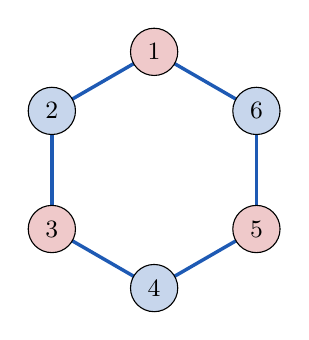
\begin{tikzpicture}[scale=1]
\coordinate (v1) at (0.000,1.500);
\coordinate (v2) at (-1.299,0.750);
\coordinate (v3) at (-1.299,-0.750);
\coordinate (v4) at (-0.000,-1.500);
\coordinate (v5) at (1.299,-0.750);
\coordinate (v6) at (1.299,0.750);
\draw[edge] (v1)--(v2);
\draw[edge] (v2)--(v3);
\draw[edge] (v3)--(v4);
\draw[edge] (v4)--(v5);
\draw[edge] (v5)--(v6);
\draw[edge] (v6)--(v1);
\node[lab,fill=RamRed!25] at (v1) {1};
\node[lab,fill=RamBlue!25] at (v2) {2};
\node[lab,fill=RamRed!25] at (v3) {3};
\node[lab,fill=RamBlue!25] at (v4) {4};
\node[lab,fill=RamRed!25] at (v5) {5};
\node[lab,fill=RamBlue!25] at (v6) {6};
\end{tikzpicture}\end{center}
\Question{Why do alternating colors work on $C_6$? What goes wrong on an odd cycle?}
\end{frame}
\begin{frame}{Odd Cycles Need a Third Color}
\large
\begin{center}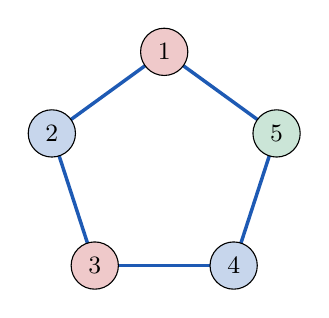
\begin{tikzpicture}[scale=1]
\coordinate (v1) at (0.000,1.500);
\coordinate (v2) at (-1.427,0.464);
\coordinate (v3) at (-0.882,-1.214);
\coordinate (v4) at (0.882,-1.214);
\coordinate (v5) at (1.427,0.464);
\draw[edge] (v1)--(v2);
\draw[edge] (v2)--(v3);
\draw[edge] (v3)--(v4);
\draw[edge] (v4)--(v5);
\draw[edge] (v5)--(v1);
\node[lab,fill=RamRed!25] at (v1) {1};
\node[lab,fill=RamBlue!25] at (v2) {2};
\node[lab,fill=RamRed!25] at (v3) {3};
\node[lab,fill=RamBlue!25] at (v4) {4};
\node[lab,fill=MapGreen!25] at (v5) {5};
\end{tikzpicture}\end{center}
\Thm{Cycle chromatic numbers}{For $n\ge3$,\[\chi(C_n)=\begin{cases}2,&n\text{ even},\\3,&n\text{ odd}.\end{cases}\]}
\end{frame}
\begin{frame}{Theorem: Two Colors and Bipartite Graphs}
\large
\Thm{Equivalent conditions}{A graph is $2$-colorable exactly when it is bipartite. This is also equivalent to having no odd cycle.}
\Proof{The two color classes are independent sets, so they form a bipartition. Conversely, color the two parts differently.\gap A cycle in a bipartite graph alternates between the two parts and is therefore even.}
\end{frame}
\begin{frame}{Proof Continued: No Odd Cycle Gives Two Colors}
\large
\Proof{Work in one connected component and choose a root $r$. Color a vertex by the parity of its distance from $r$.\gap Suppose an edge joined two vertices of the same parity. Their root paths, after removing a common initial portion, together with that edge contain an odd cycle.\gap Thus every edge joins opposite colors. Repeat in each component.\hfill$\square$}
\end{frame}
\begin{frame}{Color Classes and Independent Sets}
\large
\Def{Color class}{All vertices assigned one particular color. Every color class is independent.}
\gap A $k$-coloring partitions $V(G)$ into at most $k$ independent sets.
\gap Equivalently, coloring asks how few independent sets are needed to cover the vertices.
\end{frame}
\begin{frame}{Definition: Clique Number}
\large
\Def{Clique}{A set of pairwise adjacent vertices.}
\Def{Clique number}{The maximum size of a clique is $\omega(G)$.}
\Thm{Lower bound}{\[\chi(G)\ge\omega(G).\]}
Every vertex of a clique must have a different color.
\end{frame}
\begin{frame}{A Clique Bound Need Not Be Exact}
\large
\begin{center}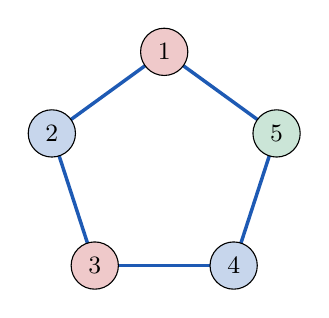
\begin{tikzpicture}[scale=1]
\coordinate (v1) at (0.000,1.500);
\coordinate (v2) at (-1.427,0.464);
\coordinate (v3) at (-0.882,-1.214);
\coordinate (v4) at (0.882,-1.214);
\coordinate (v5) at (1.427,0.464);
\draw[edge] (v1)--(v2);
\draw[edge] (v2)--(v3);
\draw[edge] (v3)--(v4);
\draw[edge] (v4)--(v5);
\draw[edge] (v5)--(v1);
\node[lab,fill=RamRed!25] at (v1) {1};
\node[lab,fill=RamBlue!25] at (v2) {2};
\node[lab,fill=RamRed!25] at (v3) {3};
\node[lab,fill=RamBlue!25] at (v4) {4};
\node[lab,fill=MapGreen!25] at (v5) {5};
\end{tikzpicture}\end{center}
For $C_5$, the largest clique has size $2$, but $\chi(C_5)=3$.
\gap A graph can require more colors than any one clique does.
\end{frame}
\begin{frame}{A Lower Bound from Independence Number}
\large
\Thm{Independence bound}{For a graph with $n$ vertices,\[\chi(G)\ge\left\lceil\frac{n}{\alpha(G)}\right\rceil.\]}
\Proof{Each color class has at most $\alpha(G)$ vertices. With $k$ classes, $n\le k\alpha(G)$. Rearrange and use integrality.\hfill$\square$}
\end{frame}
\begin{frame}{Greedy Coloring}
\large
\Def{Greedy algorithm}{Order the vertices $v_1,\ldots,v_n$. At step $i$, give $v_i$ the smallest positive integer not already used on its colored neighbors.}
\gap The output is always a proper coloring.
\gap The number of colors can depend on the ordering.
\end{frame}
\begin{frame}{Greedy Coloring: A Bad Order}
\large
Let $P_4$ have edges $ab,bc,cd$. Use the order $a,d,b,c$.
\begin{center}\begin{tabular}{ccl}\toprule Step&Vertex&Assigned color\\\midrule1&$a$&1\\2&$d$&1\\3&$b$&2\\4&$c$&3\\\bottomrule\end{tabular}\end{center}
\gap The graph needs only two colors, but this ordering makes greedy use three.
\end{frame}
\begin{frame}{Theorem: The Maximum-Degree Bound}
\large
\Thm{Greedy bound}{\[\chi(G)\le\Delta(G)+1.\]}
\Proof{When a vertex is colored, at most $\Delta(G)$ of its neighbors have already been colored. They forbid at most $\Delta(G)$ colors, leaving one of the first $\Delta(G)+1$ colors available.\hfill$\square$}
\end{frame}
\begin{frame}{A Better Bound from a Good Ordering}
\large
\Thm{Ordering bound}{If every vertex has at most $d$ earlier neighbors in an ordering, greedy coloring uses at most $d+1$ colors.}
\gap One way to find such an ordering is to repeatedly delete a vertex of degree at most $d$, then reverse the deletion order.
\gap The degree condition must hold in every remaining subgraph.
\end{frame}
\begin{frame}{Brooks' Theorem}
\large
\Thm{Brooks}{If $G$ is connected and is neither a complete graph nor an odd cycle, then\[\chi(G)\le\Delta(G).\]}
\gap Complete graphs and odd cycles show why exceptions are needed.
\gap This is a stronger theorem than the greedy bound; we state it without its full proof.
\end{frame}
\begin{frame}{Definition: Critical Graph}
\large
\Def{$k$-critical}{A graph $G$ with $\chi(G)=k$ such that every proper subgraph has chromatic number less than $k$.}
\gap Every graph of chromatic number $k$ contains a $k$-critical subgraph: keep deleting vertices or edges whenever doing so preserves the chromatic number.
\end{frame}
\begin{frame}{Critical Graphs Have Large Minimum Degree}
\large
\Thm{Critical-degree bound}{A $k$-critical graph satisfies $\delta(G)\ge k-1$.}
\Proof{If some vertex $v$ had degree at most $k-2$, color $G-v$ with at most $k-1$ colors. At most $k-2$ colors appear on the neighbors of $v$, so a color remains for $v$.\gap This produces a $(k-1)$-coloring of $G$, a contradiction.\hfill$\square$}
\end{frame}
\begin{frame}{Combining Upper and Lower Bounds}
\large
\Example{Suppose $G$ has $12$ vertices, $\alpha(G)=4$, and $\Delta(G)=3$. Then\[3\le\chi(G)\le4.\]If $G$ is connected and is not $K_4$, Brooks' theorem improves the upper bound to $3$, unless it is an odd cycle. Here its order rules out that exception. Thus $\chi(G)=3$.}
\end{frame}
\begin{frame}{Map Coloring and Planar Graphs}
\large
Represent each country by a vertex. Join two vertices when the countries share a boundary segment.
\gap Meeting only at a point does not require different colors.
\gap In the usual setting of connected countries, map coloring becomes a planar vertex-coloring problem.
\end{frame}
\begin{frame}{Theorem: Six Colors Suffice}
\large
\Thm{Six Color Theorem}{Every simple planar graph is $6$-colorable.}
\Proof{Induct on the number of vertices. A planar graph has a vertex $v$ of degree at most five. Color $G-v$ with six colors by induction. Its neighbors use at most five colors, leaving a color for $v$.\hfill$\square$}
\end{frame}
\begin{frame}{Toward Five Colors}
\large
The same induction immediately works if $\deg(v)\le4$.
\gap If $\deg(v)=5$ but two neighbors have the same color, it also works.
\Question{What if the five neighbors use all five colors? Can we change part of the coloring?}
\end{frame}
\begin{frame}{Definition: A Two-Color Component}
\large
\Def{Two-color component}{Take the subgraph induced by vertices with two chosen colors. A connected component of this subgraph is often called a Kempe component.}
\gap Interchanging the two colors throughout one component preserves properness.
\gap Edges within the component still have different endpoint colors; edges leaving it cannot cause a conflict in those two colors.
\end{frame}
\begin{frame}{Theorem: Five Colors Suffice}
\large
\Thm{Five Color Theorem}{Every simple planar graph is $5$-colorable.}
\gap Induct on $n$. Delete a vertex $v$ of degree at most five and color the rest.
\gap Only the case of five neighbors with five distinct colors needs work. List these neighbors in cyclic order as $v_1,\ldots,v_5$, with respective colors $1,\ldots,5$.
\end{frame}
\begin{frame}{Proof: The First Color Swap}
\large
\Proof{Consider colors $1$ and $3$. If $v_1$ and $v_3$ lie in different two-color components, swap colors $1$ and $3$ in the component containing $v_1$.\gap No neighbor of $v$ now has color $1$. Give that color to $v$.\gap Otherwise, there is a path of colors $1,3$ joining $v_1$ to $v_3$. We consider the second pair of colors.}
\end{frame}
\begin{frame}{Proof Continued: The Planar Separation}
\large
\begin{center}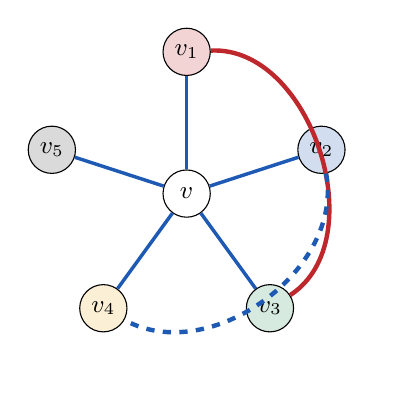
\begin{tikzpicture}[scale=1]\node[lab](v)at(0,0){$v$};\foreach \i/\a/\c in {1/90/RamRed,2/18/RamBlue,3/-54/MapGreen,4/-126/MapGold,5/162/DarkGray}{\node[lab,fill=\c!20](n\i)at(\a:1.8){$v_\i$};\draw[edge](v)--(n\i);}\draw[RamRed,line width=1.6pt](n1)to[bend left=75](n3);\draw[RamBlue,dashed,line width=1.6pt](n2)to[bend left=65](n4);\end{tikzpicture}\end{center}
A simple $1$--$3$ path, together with $vv_1$ and $vv_3$, forms a closed curve.
\gap The cyclic order puts $v_2$ and $v_4$ on opposite sides of it.
\end{frame}
\begin{frame}{Proof Continued: The Second Color Swap}
\large
\Proof{A path of colors $2,4$ from $v_2$ to $v_4$ would have to cross the closed curve. It cannot share a vertex with its $1,3$ path, and it cannot pass through the deleted vertex $v$. Planarity therefore forbids such a path.\gap Swap colors $2$ and $4$ in the component containing $v_2$. Color $2$ becomes available for $v$. The induction is complete.\hfill$\square$}
\end{frame}
\begin{frame}{The Four Color Theorem}
\large
\Thm{Four Color Theorem}{Every simple planar graph is $4$-colorable.}
\gap This is considerably harder than the Five Color Theorem; we will use it as a theorem without proving it.
\begin{center}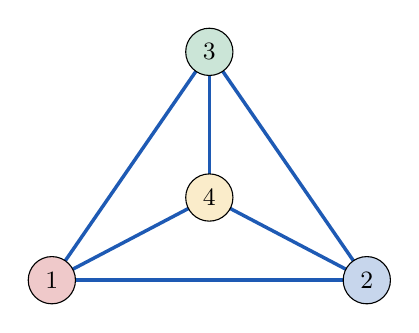
\begin{tikzpicture}[scale=1]
\coordinate (v1) at (-2.000,-1.300);
\coordinate (v2) at (2.000,-1.300);
\coordinate (v3) at (0.000,1.600);
\coordinate (v4) at (0.000,-0.250);
\draw[edge] (v1)--(v2);
\draw[edge] (v1)--(v3);
\draw[edge] (v1)--(v4);
\draw[edge] (v2)--(v3);
\draw[edge] (v2)--(v4);
\draw[edge] (v3)--(v4);
\node[lab,fill=RamRed!25] at (v1) {1};
\node[lab,fill=RamBlue!25] at (v2) {2};
\node[lab,fill=MapGreen!25] at (v3) {3};
\node[lab,fill=MapGold!25] at (v4) {4};
\end{tikzpicture}\end{center}
$K_4$ shows that four colors are sometimes necessary.
\end{frame}
\begin{frame}{Definition: Chromatic Polynomial}
\large
\Def{Chromatic polynomial}{For a positive integer $k$, let $P_G(k)$ be the number of proper colorings of $G$ using the labeled colors $1,\ldots,k$.}
\gap All $k$ colors need not be used.
\gap We will see that this counting function is a polynomial in $k$.
\end{frame}
\begin{frame}{First Chromatic Polynomials}
\large
\begin{itemize}\setlength{\itemsep}{.25cm}
\item For an edgeless graph on $n$ vertices: $P_G(k)=k^n$.
\item For $K_n$: $P_{K_n}(k)=k(k-1)\cdots(k-n+1)$.
\item For a path on $n\ge1$ vertices: $P_{P_n}(k)=k(k-1)^{n-1}$.
\end{itemize}
\gap Color a first vertex, then make the remaining choices in sequence.
\end{frame}
\begin{frame}{The Chromatic Polynomial of a Tree}
\large
\Thm{Tree formula}{For every tree $T$ with $n$ vertices,\[P_T(k)=k(k-1)^{n-1}.\]}
\Proof{Root the tree and order parents before children. The root has $k$ choices. Each other vertex need only avoid its parent's color, leaving $k-1$ choices. Unique root paths ensure that there are no other earlier neighbors.\hfill$\square$}
\end{frame}
\begin{frame}{Deletion and Contraction}
\large
\Def{Deletion $G-e$}{Remove an edge $e=uv$.}
\Def{Contraction $G/e$}{Identify $u$ and $v$ into a single vertex. Remove duplicate edges if they arise.}
\gap A coloring of $G-e$ either gives $u,v$ different colors or gives them the same color.
\end{frame}
\begin{frame}{Theorem: Deletion--Contraction}
\large
\Thm{Deletion--contraction}{For any edge $e$ of a simple graph,\[P_G(k)=P_{G-e}(k)-P_{G/e}(k).\]}
\Proof{Colorings of $G-e$ with different colors at the endpoints of $e$ are exactly the colorings of $G$. Those with equal endpoint colors correspond bijectively to colorings of $G/e$. These two classes partition the colorings of $G-e$.\hfill$\square$}
\end{frame}
\begin{frame}{Example: A Triangle}
\large
Delete one edge of $K_3$. The result is $P_3$; contraction produces $K_2$.
\begin{align*}P_{K_3}(k)&=k(k-1)^2-k(k-1)\\&=k(k-1)(k-2).\end{align*}
\gap This agrees with assigning three different colors to three mutually adjacent vertices.
\end{frame}
\begin{frame}{Example: A Four-Cycle}
\large
Deleting an edge of $C_4$ gives $P_4$; contracting it gives $K_3$.
\begin{align*}P_{C_4}(k)&=k(k-1)^3-k(k-1)(k-2)\\&=k(k-1)(k^2-3k+3).\end{align*}
\gap In particular, $P_{C_4}(2)=2$ and $P_{C_4}(3)=18$.
\end{frame}
\begin{frame}{The Chromatic Polynomial of a Cycle}
\large
\Thm{Cycle formula}{For $n\ge3$,\[P_{C_n}(k)=(k-1)^n+(-1)^n(k-1).\]}
\Proof{The formula holds for $n=3$. For $n\ge4$, deletion--contraction gives\[P_{C_n}(k)=k(k-1)^{n-1}-P_{C_{n-1}}(k).\]Insert the induction hypothesis and simplify.\hfill$\square$}
\end{frame}
\begin{frame}{Why It Is a Polynomial}
\large
\Proof{Induct using deletion--contraction. An edgeless graph has polynomial $k^n$. Deletion removes an edge, while contraction decreases the number of vertices. Thus the recurrence eventually reaches edgeless graphs.\gap At each stage we subtract two polynomials, so $P_G(k)$ is a polynomial. Its leading term is $k^n$.\hfill$\square$}
\end{frame}
\begin{frame}{Information Encoded by the Polynomial}
\large
For a simple graph of order $n$ and size $m$,
\[P_G(k)=k^n-mk^{n-1}+\text{terms of lower degree}.\]
\gap The chromatic number is the smallest positive integer $k$ for which $P_G(k)>0$.
\gap Different graphs can have the same chromatic polynomial: all trees on $n$ vertices do.
\end{frame}
\begin{frame}{Practice: Chromatic Polynomials}
\large
\Question{A graph consists of a triangle with a leaf attached to one vertex. Find its chromatic polynomial and chromatic number.}
\gap First color the triangle. Then color the leaf.
\end{frame}
\begin{frame}{Practice: Answer}
\large
\[P_G(k)=k(k-1)(k-2)(k-1)=k(k-1)^2(k-2).\]
\gap The triangle needs three colors and the leaf needs no additional color, so $\chi(G)=3$.
\gap This combines a local structural observation with the product rule.
\end{frame}
\begin{frame}{Summary: Colorings}
\large
\begin{itemize}\setlength{\itemsep}{.23cm}
\item Color classes are independent sets.
\item Cliques and independence number give lower bounds; greedy coloring gives upper bounds.
\item Planarity implies five colors by a short recoloring proof, and four by a deeper theorem.
\item Chromatic polynomials count labeled proper colorings; deletion--contraction computes them.
\end{itemize}
\end{frame}
\begin{frame}{Next time: Matchings}\begin{center}{\Huge Matchings}\end{center}\end{frame}
\end{document}